\documentclass{article}
\usepackage{graphicx} % Required for inserting images
\graphicspath{ {./images/} }
\graphicspath{ {images/} }
\usepackage{xcolor}
\usepackage{amsmath}
\usepackage{multicol}
\usepackage{amsmath}
\usepackage{amsfonts}
\usepackage{amssymb}
\usepackage{url}
\usepackage{mdframed}
\usepackage{hyperref}
\usepackage{subfigure}
\usepackage{fancybox,graphicx}
\usepackage{mathrsfs} 
\usepackage{amsfonts}
\usepackage{longtable,array}
\usepackage{multirow}
\usepackage[latin1]{inputenc}
\usepackage[T1]{fontenc}
\usepackage{array}
\usepackage{booktabs}

\usepackage{hyperref}
\newmdenv[linecolor=black,skipabove=\topsep,skipbelow=\topsep,
leftmargin=-5pt,rightmargin=-5pt,
innerleftmargin=5pt,innerrightmargin=5pt]{mybox}
\usepackage[a4paper,left=22mm,top=20mm,right=22mm]{geometry}

\title{Techniques of Integration}
\author{USTH LEARNING SUPPORT}
\date{December 2023}
\begin{document}
\maketitle
\tableofcontents
\newpage
\section{Using Basic Integration Formulas and Substitution Rule}
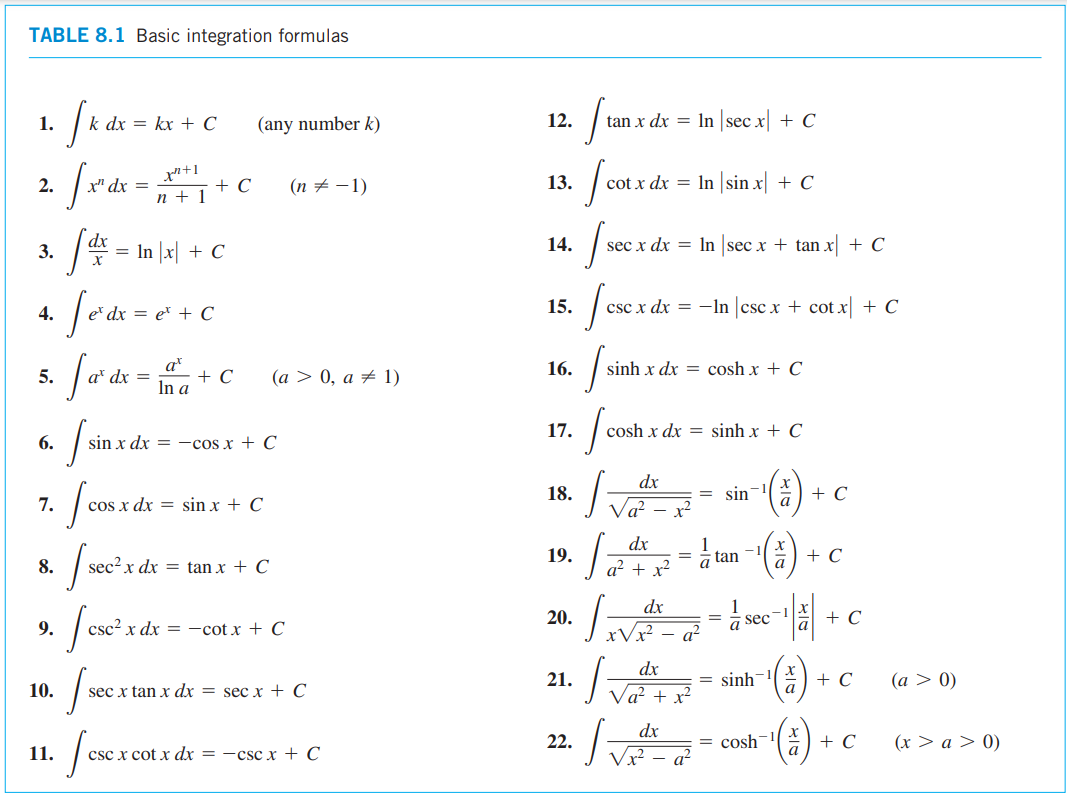
\includegraphics[width=1\linewidth]{formula.png}
\textbf{Substitution Rule for definite integrals:} If g'(x) is continuous on [a,b] and f is continuous on the range of u=g(x), then:
     \begin{center}
         \begin{equation*}
            \displaystyle\int\limits_{a}^{b}f(g(x))g'(x)dx = \displaystyle\int\limits_{g(a)}^{g(b)}f(u) du
         \end{equation*}
     \end{center}
    Two ways to make a substitution: \\
            $+)\ u=g(x)$ \\
            $+)\ x=h(u)$ (this method will be used more in part 3,4) \\
    \textbf{Note:} Substitution Rule for indefinite integrals is the same as Substitution Rule for definite integrals but there is no bounds.\\
    \textbf{Example:} Evaluate $I=\displaystyle\int\limits_{-1}^{1} 3x^2\sqrt{x^3+1}dx$\\
    \begin{equation*}
         I=\displaystyle\int\limits_{-1}^{1} 3x^2\sqrt{x^3+1}dx = \displaystyle\int\limits_{-1}^{1}(x^3+1)'\sqrt{x^3+1}dx = \displaystyle\int\limits_{-1}^{1} \sqrt{x^3+1}d(x^3+1)
    \end{equation*}
    \text{Let $u = g(x) = x^3+1$}\\
    =$>$ $g(-1)=0$ and $g(1)=2$\\
    =$>$ I = $\displaystyle\int\limits_{0}^{2}\sqrt{u}du = \displaystyle\int\limits_{0}^{2} u^\frac{1}{2}du=\left[\displaystyle\frac{2}{3}u^\frac{3}{2}\right]_0^2 = \frac{2}{3}.2\sqrt{2} = \frac{4\sqrt{2}}{3}$\\
\newpage
    \textbf{Example:} Evaluate $I=\displaystyle\int\limits_{\pi/4}^{\pi/2} \frac{cos\ x}{\sin\ x}dx$\\
    \begin{equation*}
        I = \displaystyle\int\limits_{\pi/4}^{\pi/2} \frac{cos\ x}{\sin\ x}dx =\displaystyle\int\limits_{\pi/4}^{\pi/2}\frac{(\sin\ x)'}{\sin\ x}dx=\displaystyle\int\limits_{\pi/4}^{\pi/2}\frac{d(\sin\ x)}{\sin\ x}
    \end{equation*}
    Let $u = g(x) = \sin x$\\
    =$>$ $g(\displaystyle\frac{\pi}{4})=\displaystyle\frac{\sqrt{2}}{2}\ and\ g\displaystyle(\frac{\pi}{2}) = 1$\\
    =$>$ I = $\displaystyle\int\limits_{\frac{\sqrt{2}}{2}}^{1}\displaystyle\frac{du}{u}=\left[ln|u|\right]_{\frac{\sqrt{2}}{2}}^{1}=-ln\displaystyle\frac{\sqrt{2}}{2}$
\section{Integration by Parts}
Integration by Parts for definte integrals: If f and g are both differentiable, then:
\begin{equation*}
    \displaystyle\int\limits_{a}^b f(x)g'(x)dx=\left[f(x)g(x)\right]_{a}^{b} - \displaystyle\int\limits_{a}^{b} f'(x)g(x)dx
\end{equation*}
Or it can be written as:\\
$$
     \displaystyle\int\limits_{a}^{b}udv= \left[uv\right]_{a}^{b}-\displaystyle\int\limits_{a}^{b}vdu
$$
\textbf{Note: }Integration by Parts for \textbf{indefinite} integrals is the same as Integration by Parts for \textbf{definite}\\integrals but there is no bounds.\\
\textbf{Tips to choose u and dv:}\ we usually choose \textbf{u}  in order of priority: \\
\begin{center}
    logarithmic function -$>$ polynomial function -$>$ trigonometric function/exponential function
\end{center}
and the rest is \textbf{dv}.\\
In some cases, we should choose \textbf{dv} that we can easily determine \textbf{v} from \textbf{dv}\\
\\
\textbf{Example: } Determine I=$\int x^2e^xdx$ \\
We can see that $x^2$ is a polynomial function and $e^x$ is a exponential function so we choose u= $x^2$ and dv=$e^x$dx\\
Apply integration by Parts\\
Choose u=$x^2$ =$>$ du=2x\ dx\\
.\quad \quad \quad dv=$e^x$dx =$>$ dv=d($e^x$) =$>$ v=$e^x$
\begin{equation*}
    I= x^2e^x - \int e^x 2xdx
\end{equation*}
The new integral is less complicated than the original because the exponent on x is reduced
by one.
Apply integration by Parts for the integral on the right:
\begin{flalign*}
    u=2x \Rightarrow du=2dx\\
dv=e^xdx \Rightarrow v=e^x &&\\
\Rightarrow\ \int e^x 2xdx =&\ 2xe^x - 2\int e^xdx \\= &\ 2xe^x - 2e^x +C\\
\Rightarrow\ I =&\ x^2e^x - 2xe^x + 2e^x +C&&\\
\end{flalign*}
\textbf{Example: } I = $\int\limits_{0}^{4}xe^{-x}dx$ \\
Apply Integration by Parts:
\begin{flalign*}
   Choose\ &u=x \Rightarrow\ du=dx\\
&dv=e^{-x}dx\ \Rightarrow\ v=-e^{-x}&&\\ 
   \Rightarrow\  I=&\left[-xe^{-x}\right]_{0}^{4}+ \int\limits_{0}^{4} e^{-x}dx \\=& -4e^{-4}-\int\limits_{0}^{4} e^{-x}d(-x)\\ =& -4e^{-4}- \left[e^{-x}\right]_{0}^{4}\\ =& -5e^{-4} +1&&\\ 
\end{flalign*}
\textbf{Example: } I=$\int ln\ x\ dx$\\
Apply Integration by Parts:
\begin{flalign*}
   Choose\ &u=ln\ x\ \Rightarrow\ du=\displaystyle\frac{1}{x}dx\\
&dv=1.dx\ \Rightarrow\ v=x&&\\
\Rightarrow\ I=&\ xln\ x - \displaystyle\int x.\frac{1}{x}dx \\
=&\ xln\ x-x+C &&
\end{flalign*}
\section{Trigonometric Integrals}
\subsection{Evaluating $\int\sin^m x\ cos^n x\ dx$}
    \begin{center}
        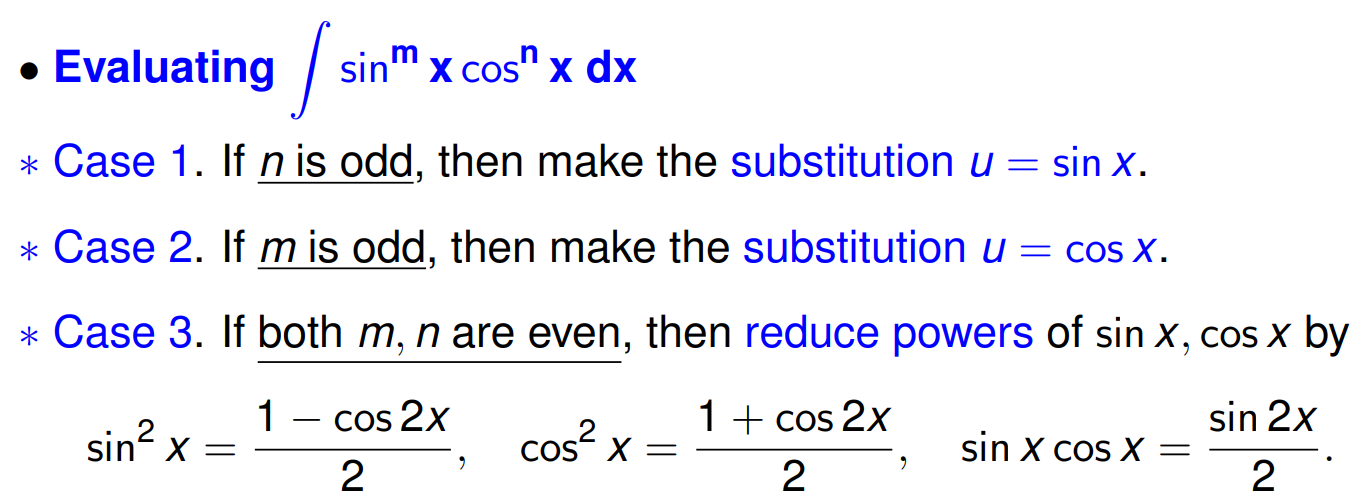
\includegraphics[width=1\linewidth]{sin cos.png}
        \label{fig:enter-label}
    \end{center}
\textbf{Tips to remember case 1,2: }If the exponent of $\sin$ x is odd then substitute u=cos x, if the exponent of cos x is odd then substitute $u=\sin x$.\\
\textbf{Example: } Determine I=$\int \sin^3x\ cos^2x\ dx$\\
(We can see that the exponent of sin x is odd, then substitute u=cos x)\\
Let u=cos x\\
=$>$ $du=d(cos x)=-\sin x\ dx$\\
=$>$ $dx=-\displaystyle\frac{du}{\sin x}$\\
\begin{flalign*}
    \Rightarrow\ I= &\displaystyle\int\frac{-u^2\sin^3x\ du}{\sin x}\\
    = &-\int u^2 \sin^2x\ du \\
    = &-\int u^2(1-u^2)du \\
    = &\int u^4 - u^2 du\\
    = &\ \frac{u^5}{5}-\frac{u^3}{3}+C\\
\Rightarrow\ I = &\ \displaystyle\frac{cos^5x}{5}-\frac{cos^3x}{3} +C&&
\end{flalign*}
\textbf{Example: } Determine $I=\int cos^3x\ dx$\\
(We can see that the exponent of cos x is odd, and the exponent of sin x is even (0), so we substitute u=sin x)\\
Let u=sin x\\
=$>$ $du= cos\ x\ dx$\\
=$>$ $dx=\displaystyle\frac{du}{cos\ x}$
\begin{flalign*}
    \Rightarrow\ I=&\int cos^2x\ du \\
    =&\ \int (1-u^2)du \\
    =&\ u-\displaystyle\frac{u^3}{3}+C\\
\Rightarrow\ I=&\sin\ x - \displaystyle\frac{\sin^3 x}{3}+C&&\\
\end{flalign*}
\textbf{Example: }Determine $I=\int \sin^4x\ cos^2x\ dx$\\
(We can see that the exponents of sin x and cos x are even)
\begin{flalign*}
    I= &\ \displaystyle\int (\sin^2x)^2\ cos^2x\ dx \\
    =&\ \int\left(\frac{1-cos 2x}{2}\right)^2.\frac{1+cos 2x}{2}dx\\
    =&\ \frac{1}{8}\int(1-2cos\ 2x+cos^22x)(1+cos\ 2x)dx\\
=&\ \displaystyle\frac{1}{16}\int (1+cos\ 2x-2cos\ 2x-2cos^22x+cos^22x+cos^32x)d(2x)\\
=&\ \displaystyle\frac{1}{16}\left(2x+\sin\ 2x-2\sin\ 2x-\int cos^22x\ d(2x) +\int cos^32x\ d(2x)\right)&&
\end{flalign*}

Let u=2x, we have:\\
$I=\displaystyle\frac{1}{16} \left(u+\sin\ u-2\sin\ u -\int cos^2 u\ du+\int cos^3u\ du \right) $\\
I will let these two integrals be an exercise for you, practice makes perfect :)\\
=$>$ $I= \displaystyle\frac{1}{16}\left(u+\sin\ u-2\sin\ u -\frac{1}{2}u-\frac{1}{4}\sin\ 2u+\sin\ u-\frac{\sin^3u}{3}\right)+C$\\
=$>$ $I=\displaystyle\frac{x}{16}-\frac{1}{64}\sin\ 4x-\ \frac{1}{48}\sin^32x+C $
\subsection{Evaluating $\int tan^m\ xsec^n x\ dx$}
\begin{center}
    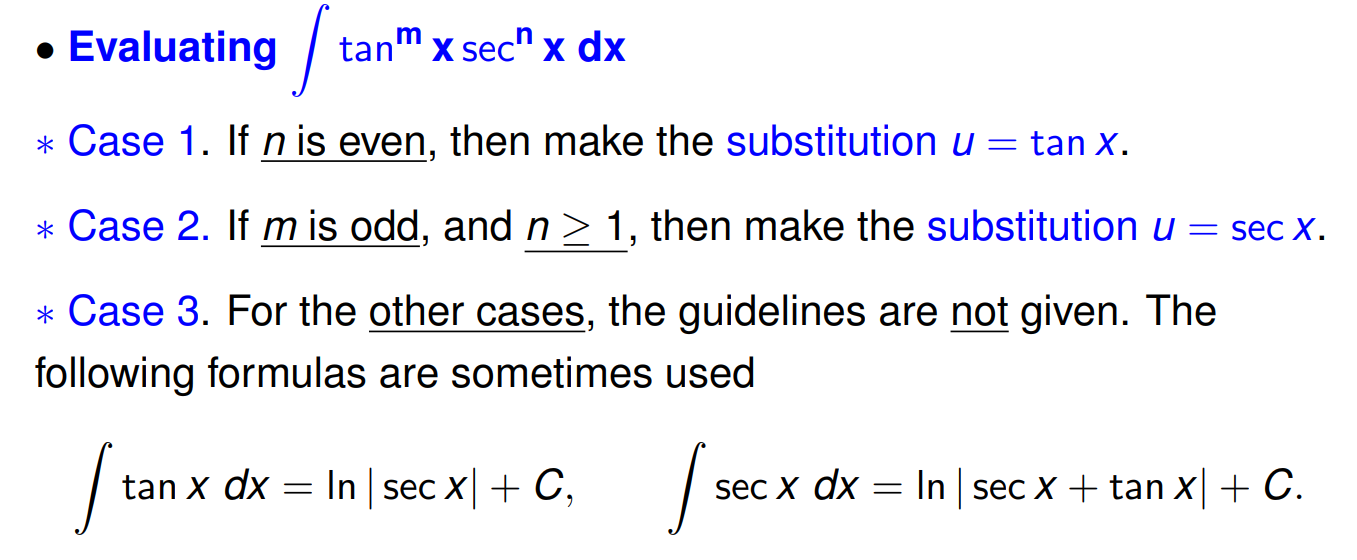
\includegraphics[width=1\linewidth]{tan sec.png}
    \label{fig:enter-label}
\end{center}
\textbf{Some trigonometric equations you may need:}\\
1) $tan^2 x =sec^2x-1$\\
2) $sec^2x=tan^2x+1$\\
3) $sec^2x-tan^2x=1$\\
(Actually these three equations are the same :))\\
\textbf{Example}: Evaluate $I=\int\tan^3x\ sec^2x\ dx$\\
(We can see that the exponent of tan\ x is odd and the exponent of sec\ x is even and $\geq 1$ so you can choose the way you like to substitute u)\\
+) Method 1:\\
Let u=tan x\\
=$>$ $du=\displaystyle\frac{dx}{cos^2x}$
=$>$ $dx=cos^2x\ du$
\begin{flalign*}
    \Rightarrow\ I=& \displaystyle\int u^3sec^2x\ cos^2x\ du\\
    = &\ \int u^3du=\frac{u^4}{4}+ C\\
\Rightarrow\ I=&\ \displaystyle\frac{tan^4x}{4}+C&&
\end{flalign*}
+) Method 2: (You should try to use this method before seeing my solution to see whether your result is the same as the result of method 1)\\
Let u=sec x\\
=$>$ $du=sec\ x\ tan\ x\ dx$
=$>$ $dx=\displaystyle\frac{du}{u.tan\ x}$
\begin{flalign*}
    \Rightarrow\ I=&\ \displaystyle\int\frac{tan^3x\ u^2\ du}{u.tan\ x}\\
    = &\ \int u.tan^2x\ du\\
    =&\ \int u(u^2-1)du\\
    =&\ \int (u^3-u)du=\frac{u^4}{4}-\frac{u^2}{2}+C\\
\Rightarrow\ I=&\ \displaystyle\frac{sec^4x}{4}-\frac{sec^2x}{2}+C&&
\end{flalign*}

At the first look, you may be confused because those results do not seem similar and you think you have made some mistakes.\\
I will prove those results are similar:\\
\begin{flalign*}
    \displaystyle\frac{sec^4x}{4}-\frac{sec^2x}{2}+C=& \ \frac{(sec^2x)^2-2sec^2x}{4}+C\\
    =&\ \frac{(1+tan^2x)^2-2(1+tan^2x)}{4}+C\\
    =&\ \frac{tan^4x+2tan^2x+1-2-2tan^2x}{4}+C\\
    =&\ \frac{tan^4x+1}{4}+C\\
    =&\ \frac{tan^4x}{4}+\frac{1}{4}+C\\
    =&\ \frac{tan^4x}{4}+C
\end{flalign*}
Therefore, two results are the sameeee.\\
\textbf{Example: }Evaluate $I=\int sec^3x\ dx$\\
(We can see that this problem belongs to case 3, so you have to think harder.)\\
We have: $I=\int sec\ x\ sec^2x\ dx$\\
Applying integration by Parts:\\
Choose $u=sec\ x$ $\Rightarrow$ $du=sec\ x\ tan\ x\ dx$\\
.\quad \quad \quad $dv=sec^2x\ dx=\displaystyle\frac{1}{cos^2x}dx \Rightarrow v=tan\ x$\\
\begin{flalign*}
 \Rightarrow\ I=&\ \sec\ x\ tan\ x-\displaystyle\int tan^2x\ sec\ x\ dx\\
 =&\ \sec\ x\ tan\ x-\int (\sec^2x-1)\sec\ x\ dx\\
=&\ \sec\ x\ tan\ x-\int \sec^3x\ dx+\int \sec\ x\ dx\\
=&\ \sec\ x\ tan\ x - I + ln\left|\sec\ x + \tan\ x\right|+C\\
\Rightarrow\ 2I=& \ sec\ x\ tan\ x+ln\left|\sec\ x + \tan\ x\right|+C\\
\Rightarrow\ I=&\ \displaystyle\frac{1}{2}\sec\ x\ \tan\ x+\frac{1}{2}ln\left|\sec\ x + \tan\ x\right|+C&&   
\end{flalign*}
\subsection{Evaluating products of sine and cosine $\int \sin(mx)cos(nx)dx$}
\begin{center}
 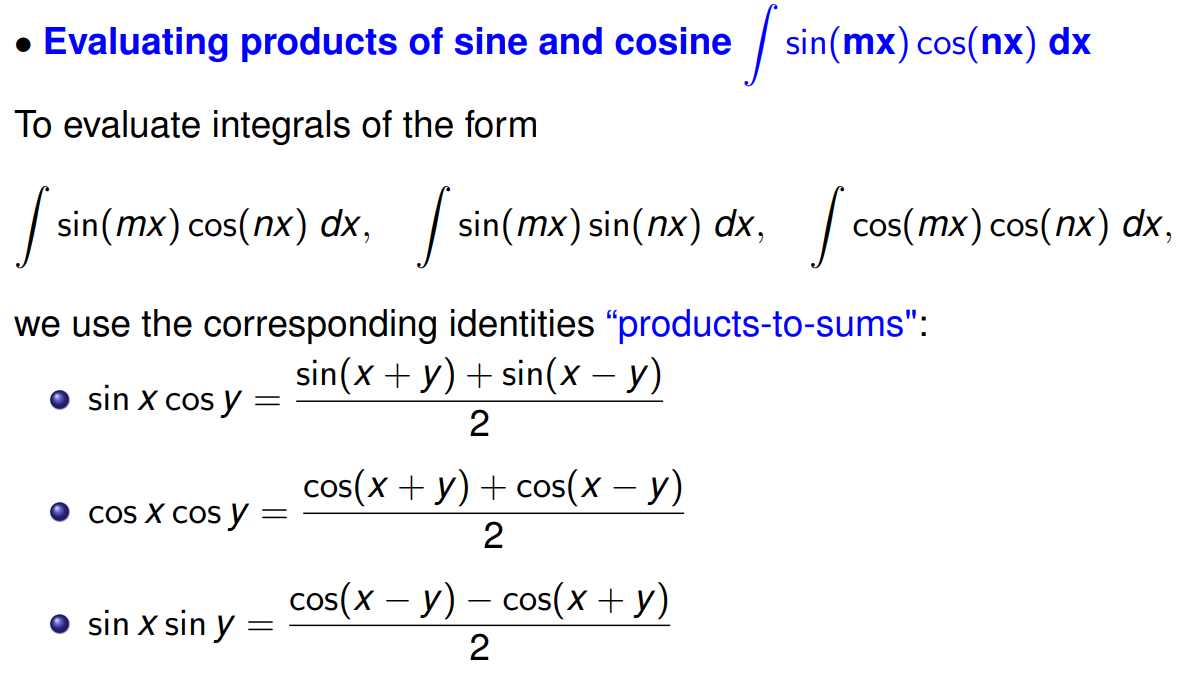
\includegraphics[width=1\linewidth]{cos sin.png}
\end{center}
\textbf{Example: }Evaluate $I=\int\limits_{0}^{\pi /2}\sin\ x\ cos\ x\ dx$
\begin{flalign*}
   I=&\ \displaystyle\frac{1}{2}\int\limits_{0}^{\pi /2}(\sin\ 2x+\sin\ 0)dx\\
   =&\ \frac{1}{4}\int\limits_{0}^{\pi /2}\sin\ 2x\ d(2x)\\
   =&\ \left[ \frac{-cos\ 2x}{4}\right]_{0}^{\pi/2}\\
   =&\ \frac{1}{2}&& 
\end{flalign*}
Another method 
\textbf{(MUST KNOW):} Using 2 sin x cos x = sin 2x\\
\textbf{Example: }Evaluate $I=\int\cos\ 3x\ cos\ 2x\ dx$
\begin{flalign*}
    I=&\ \displaystyle\frac{1}{2}\int (cos\ 5x + cos\ x) dx\\
    =&\ \frac{1}{2}\left(\frac{1}{5}\sin\ 5x+\sin\ x\right)+C\\
    =&\ \frac{1}{10}\sin\ 5x +\frac{1}{2}\sin\ x+C&&
\end{flalign*}
\textbf{Example: }Evaluate $I=\int \sin\ 5x\ \sin\ 3x\ dx$
\begin{flalign*}
    I=&\ -\displaystyle\frac{1}{2}\int (cos\ 8x-cos\ 2x)dx\\
    =&\ -\frac{1}{2}\left(\frac{1}{8}\sin\ 8x-\frac{1}{2}\sin\ 2x\right)+C\\
    =&\ -\frac{1}{16}\sin\ 8x+\frac{1}{4}\sin\ 2x+C&&
\end{flalign*}
\textbf{Example: }Evaluate $I=\int \sin^2x\ cos\ 3x\ dx$
\begin{flalign*}
    I=&\ \displaystyle\int \frac{1-cos\ 2x}{2}cos\ 3x\ dx\\
    =&\ \frac{1}{2}\int(1-cos\ 2x)cos\ 3x\ dx\\
    =&\ \frac{1}{2}\int (cos\ 3x-cos\ 3x\ cos\ 2x)dx\\
    =&\ \frac{1}{2}\left(\int cos\ 3x\ dx -\int cos\ 3x\ cos\ 2x\ dx\right) &&
\end{flalign*}
(You can calculate these integrals (section 3.1 and 3.3), so try to calculate them by yourself $<3$)\\
$I= \displaystyle\frac{1}{6}\sin\ 3x-\frac{1}{20}\sin\ 5x-\frac{1}{4}\sin\ x+ C$\\
\section{Trigonometric Substitutions}
\begin{center}
    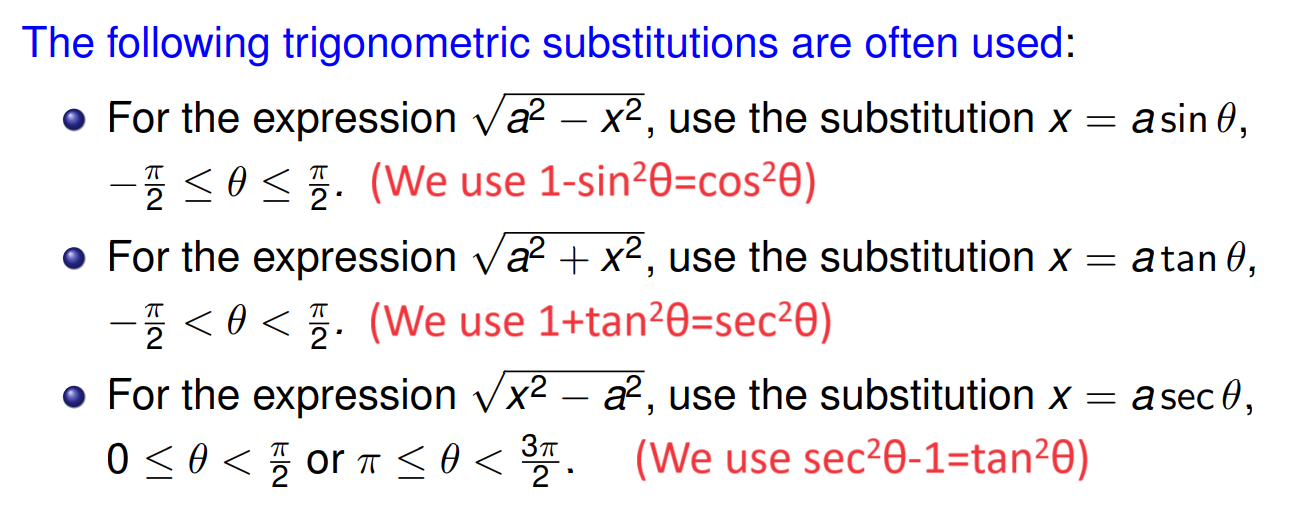
\includegraphics[width=1\linewidth]{tri.png}
\end{center}
\textbf{Example:} Evaluate $I=\displaystyle\int\frac{dx}{\sqrt{1-x^2}}$\\
Let $x=\sin\ u\ \left(u\in \left[\displaystyle\frac{-\pi}{2},\frac{\pi}{2}\right]\right)$\\
=$>$ $dx=cos\ u\ du$ and $u=arc\sin\ x$
\begin{flalign*}
    \Rightarrow\ I=&\ \displaystyle\int\frac{cos\ u\ du}{\sqrt{1-\sin^2u}}\\
    =&\ \displaystyle\int\frac{cos\ u\ du}{\sqrt{cos^2u}}\\
    =&\ \int\frac{cos\ u}{cos\ u}du\ (since\ u\in \left[\displaystyle\frac{-\pi}{2},\frac{\pi}{2}\right])\\
=&\ \int du\\
=&\ u+C\\
=&\ \arcsin\ x +C&&
\end{flalign*}
\textbf{Example: }Evaluate $I=\displaystyle\int\limits_{0}^{3}\frac{dx}{\sqrt{9+x^2}}$\\
Let $x=3tan\ u\ \left(u\in \left[\displaystyle\frac{-\pi}{2},\frac{\pi}{2}\right]\right)$\\
=$>$ $dx=\displaystyle\frac{3}{cos^2u}du=3sec^2u\ du$\\
When $x=0 \Rightarrow u=0$\\
.\quad \quad \quad $x=3 \Rightarrow u=\displaystyle\frac{\pi}{4}$
\begin{flalign*}
    \Rightarrow\ I=&\ \displaystyle\int\limits_{0}^{\pi/4}\frac{3sec^2u\ du}{\sqrt{9+9tan^2u}}=\displaystyle\int\limits_{0}^{\pi/4}\frac{3sec^2u\ du}{3\sqrt{1+tan^2u}}\\
    =&\ \displaystyle\int\limits_{0}^{\pi/4}\frac{sec^2u\ du}{\sqrt{sec^2u}}= \displaystyle\int\limits_{0}^{\pi/4}sec\ u \\
    =&\ \left[ln \left|sec\ u+tan\ u\right|\right]_{0}^{\pi/4}\\
    =&\ ln(1+\sqrt{2})&&
\end{flalign*}
\textbf{Example: }Evaluate $I=\displaystyle\int\frac{1}{\sqrt{x^2-49}}dx$\\
Let $x=7sec\ u$ $\left(u\in \left[\displaystyle 0,\frac{\pi}{2}\right)\right)$\\
=$>$ $dx=7sec\ u\ tan\ u\ du$
\begin{flalign*}
    \Rightarrow\ I=&\ \displaystyle\int\frac{7sec\ u\ tan\ u\ du}{\sqrt{49sec^2u-49}}\\
    =&\ \int\frac{7sec\ u\ tan\ u\ du}{7\sqrt{sec^2u-1}}\\
    =&\ \int\frac{sec\ u\ tan\ u\ du}{tan\ u}\\
=&\ \int sec\ u\ du=ln\left|sec\ u+tan\ u \right|+C\\
=&\ ln\left|\displaystyle\frac{x}{7}+tan\left(arcsec\frac{x}{7}\right)\right|+C&&
\end{flalign*}
\textbf{Example: }Evaluate $I=\displaystyle\int\limits_{0}^{1/3}\sqrt{1-9x^2}dx$\\
Let $x=\displaystyle\frac{1}{3}\sin\ u$ $\left(u\in \left[\displaystyle\frac{-\pi}{2},\frac{\pi}{2}\right]\right)$ =$>$ $dx=\displaystyle\frac{1}{3}cos\ u\ du$\\
When x=0 =$>$ u=0\\
.\quad \quad \quad $x=\displaystyle\frac{1}{3}$ =$>$ $u=\displaystyle\frac{\pi}{2}$
\begin{flalign*}
    \Rightarrow\ I=&\ \displaystyle\frac{1}{3}\int\limits_{0}^{\pi /2}cos\ u\sqrt{1-9.\frac{1}{9}\sin^2u}\ du=\displaystyle\frac{1}{3}\int\limits_{0}^{\pi /2}cos\ u\sqrt{cos^2u}\ du\\
    =&\ \displaystyle\frac{1}{3}\int\limits_{0}^{\pi /2}cos^2u\ du=\displaystyle\frac{1}{3}\int\limits_{0}^{\pi /2}\frac{1+cos\ 2u}{2}du\\
    =&\ \displaystyle\frac{1}{3}\int\limits_{0}^{\pi /2}\left(\frac{1}{2}+\frac{1}{2}cos\ 2u\right)du=\frac{1}{3}\left[\frac{1}{2}u+\frac{1}{4}\sin\ 2u\right]_{0}^{\pi /2}=\frac{\pi}{12}&&
\end{flalign*}
\newpage
\section{Integration of Rational Functions by Partial Fractions}
This section shows how to express a rational function $f(x)=\displaystyle\frac{p(x)}{q(x)}$ as a sum of simpler fractions, called partial fractions, which are easily integrated.\\
A rational function $f(x)=\displaystyle\frac{p(x)}{q(x)}$ is said to be \textbf{proper} if the degree of p(x) is \textbf{less} than the degree of q(x); otherwise, the rational function is \textbf{improper}\\
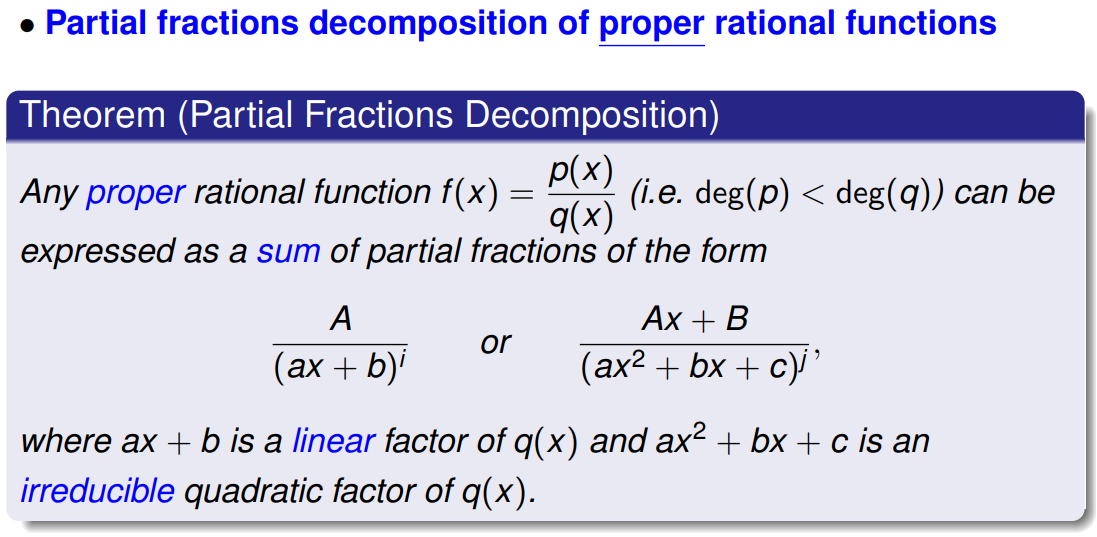
\includegraphics[width=1\linewidth]{partial.png}
\textbf{Note: }
\begin{itemize}
    \item A polynomial is said to be \textbf{irreducible} if it cannot be factorized into two.
or more polynomials (with real coefficients) of smaller degree
    \item Every polynomial of \textbf{degree $\geq$ 3} is \textbf{reducible}. We can keep factorizing a polynomial into factors of smaller degree until we reach a linear or an irreducible quadratic factor.
    \item \textbf{We can factorize a polynomial q(x) by finding its roots}.
    \item With improper rational functions $\displaystyle\frac{p(x)}{q(x)}$, perform $\displaystyle\frac{p(x)}{q(x)}=r(x)+\displaystyle\frac{s(x)}{q(x)}$\\ 
    (divide p(x) for q(x), r(x) is the result, s(x) is the remainder)
\end{itemize}
\newpage
\textbf{Steps to find the partial fractions decomposition of a rational function:}\\
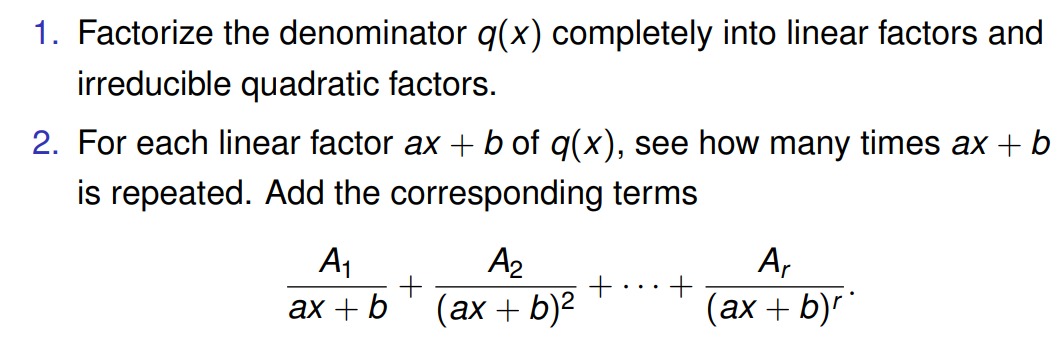
\includegraphics[width=0.75\linewidth]{step.png}\\
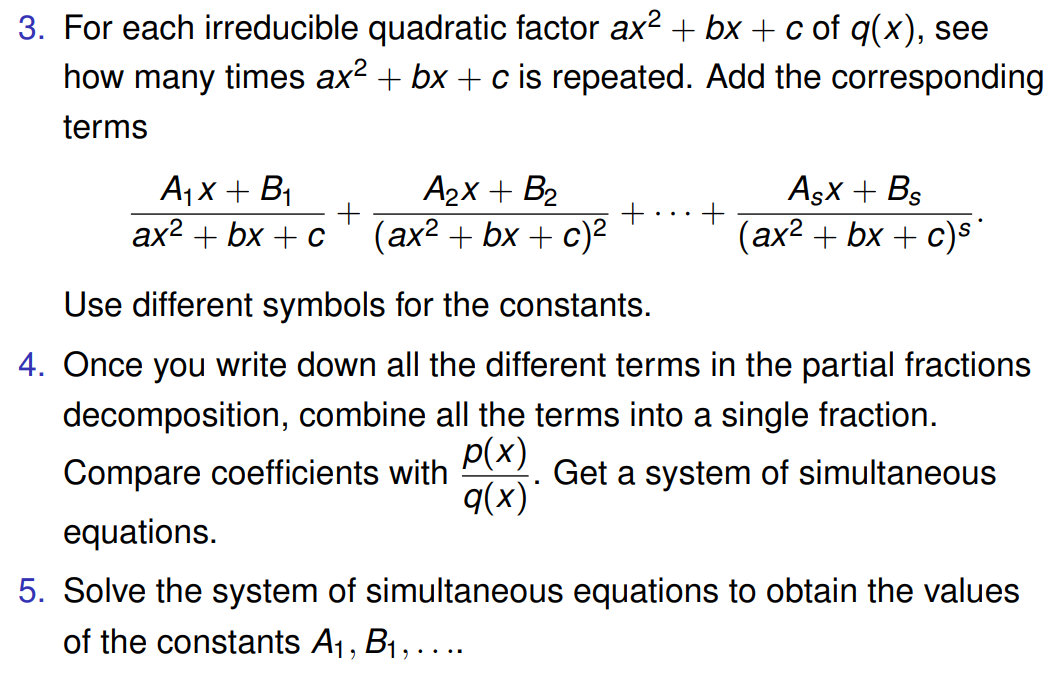
\includegraphics[width=0.75\linewidth]{step2.png}\\
\textbf{Example: }Find the partial fractions decomposition of $f(x)=\displaystyle\frac{5x-3}{x^2-2x-3}$\\
Step 1, we have to factorize $q(x)=x^2-2x-3$\\
By solving q(x)=0, q(x) has 2 roots: x=3 and x=-1\\
$\Rightarrow q(x)=x^2-2x-3=(x-3)(x+1)$\\
So q(x) is reducible, then we do not need to do step 3\\
Step 2, then f(x) can be written as:
\begin{flalign*}
    f(x)=&\ \displaystyle\frac{5x-3}{x^2-2x-3}=\frac{5x-3}{(x-3)(x+1)}\\
    =&\ \frac{A}{x-3}+\frac{B}{x+1}=\frac{A(x+1)+B(x-3)}{(x-3)(x+1)}\\
    =&\ \frac{Ax+A+Bx-3B}{(x-3)(x+1)} =\displaystyle\frac{(A+B)x+(A-3B)}{(x-3)(x+1)}\\
\Rightarrow\ f(x)=&\ \frac{5x-3}{(x-3)(x+1)}=\displaystyle\frac{(A+B)x+(A-3B)}{(x-3)(x+1)}&&
\end{flalign*}
$\Rightarrow$ Step 4, $A+B=5$ and $A-3B=-3$\\
$\Rightarrow$ Step 5, A=3 and B=2\\
$\Rightarrow\ f(x)=\displaystyle\frac{3}{x-3}+\frac{2}{x+1}$\\
\newpage
\textbf{Example: }Determine $I=\displaystyle\int\frac{x^2+4x+1}{(x-1)(x+1)(x+3)}dx$\\
\begin{flalign*}
    Consider\ f(x)=&\ \displaystyle\frac{x^2+4x+1}{(x-1)(x+1)(x+3)}\\
    =&\ \frac{A}{x-1}+\frac{B}{x+1}+\frac{C}{x+3}\\
    =&\ \frac{A(x+1)(x+3)+B(x-1)(x+3)+C(x-1)(x+1)}{(x-1)(x+1)(x+3)}\\
    =&\ \frac{(A+B+C)x^2+(4A+2B)x+(3A-3B-C)}{(x-1)(x+1)(x+3)}&&
\end{flalign*}
$\Rightarrow$ We have these equations:
\begin{flalign*}
    A+B+C=1\\
    4A+2B=4\\
    3A-3B-C=1
\end{flalign*}
$\Rightarrow\ A=\displaystyle\frac{3}{4},\ B=\frac{1}{2},\ C=\frac{-1}{4}$\\
\textbf{There is another way to calculate A,B,C\\
We can solve $A(x+1)(x+3)+B(x-1)(x+3)+C(x-1)(x+1)=x^2+4x+1 $ (1) in a way that we do not need to expand those things. That is substituting x by roots of (x+1)(x+3)(x-1), so the equation will be easier to find A,B,C.\\
If x=1, (1) becomes $8A=6$ =$>$ $A=3/4$ \\
If x=-1, (1) becomes $-4B=-2$ =$>$ $B=1/2$\\
If x=-3, (1) becomes $8C=-1$ =$>$ $C=-1/4$\\}
$\Rightarrow$ $f(x)=\displaystyle\frac{\frac{3}{4}}{x-1}+\frac{\frac{1}{2}}{x+1}+\frac{\frac{-1}{4}}{x+3}$
\begin{flalign*}
\Rightarrow\ I=&\ \displaystyle\int\left(\displaystyle\frac{\frac{3}{4}}{x-1}+\frac{\frac{1}{2}}{x+1}+\frac{\frac{-1}{4}}{x+3}\right)dx\\
=&\ \frac{3}{4}ln\left|x-1\right|+\frac{1}{2}ln\left|x+1\right|-\frac{1}{4}ln\left|x+3\right|+C&&
\end{flalign*}
\textbf{Example: }Find the partial fractions decomposition of $f(x)=\displaystyle\frac{6x+7}{x^2+4x+4}$\\
First, factorize $q(x)=x^2+4x+4=(x+2)^2$\\
We can see that $q(x)=(x+2)^2$\\ =$>$ (x+2) repeats twice.
\begin{flalign*}
    f(x)=&\ \displaystyle\frac{6x+7}{(x+2)^2}\\
    =&\ \frac{A}{x+2}+\frac{B}{(x+2)^2}\\
    =&\ \frac{A(x+2)+B}{(x+2)^2}\\
    =&\ \frac{Ax+(2A+B)}{(x+2)^2}&&
\end{flalign*}
$\Rightarrow$ $A=6,B=-5$\\
$\Rightarrow$ $f(x)=\ \displaystyle\frac{6}{x+2}-\frac{5}{(x+2)^2}$\\
\newpage
\textbf{Example: } Determine $I=\displaystyle\int\frac{8x^2+8x+2}{(4x^2+1)^2}dx$\\
Consider $f(x)=\displaystyle\frac{8x^2+8x+2}{(4x^2+1)^2}$\\
We can see that $(4x^2+1)$ repeats twice.
\begin{flalign*}
    \Rightarrow\ f(x)=&\ \displaystyle\frac{8x^2+8x+2}{(4x^2+1)^2}\\
    =&\ \frac{Ax+B}{4x^2+1}+\frac{Cx+D}{(4x^2+1)^2}\\
    =&\ \frac{(Ax+B)(4x^2+1)+Cx+D} {(4x^2+1)^2}\\
    =&\ \frac{4Ax^3+4Bx^2+Cx+(A+B+D)}{(4x^2+1)^2}&&
\end{flalign*}
$\Rightarrow\ A=0,B=2,C=8,D=0\\
\Rightarrow\ f(x)=\displaystyle\frac{2}{4x^2+1}+\frac{8x}{(4x^2+1)^2}$\\
\\
Try to determine I by yourself (hint: substitute x=1/2 tan u)\\
\\
Let's see Assoc.Prof. Le Hai Khoi's example:\\
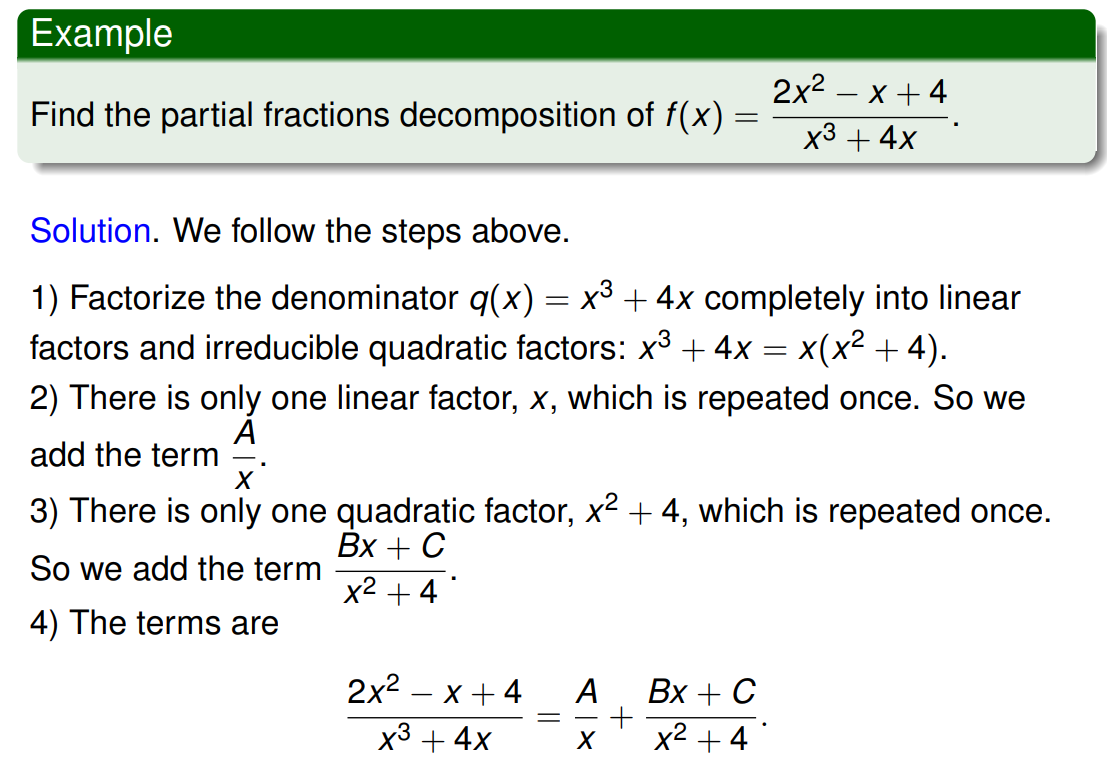
\includegraphics[width=0.59\linewidth]{ex.png} 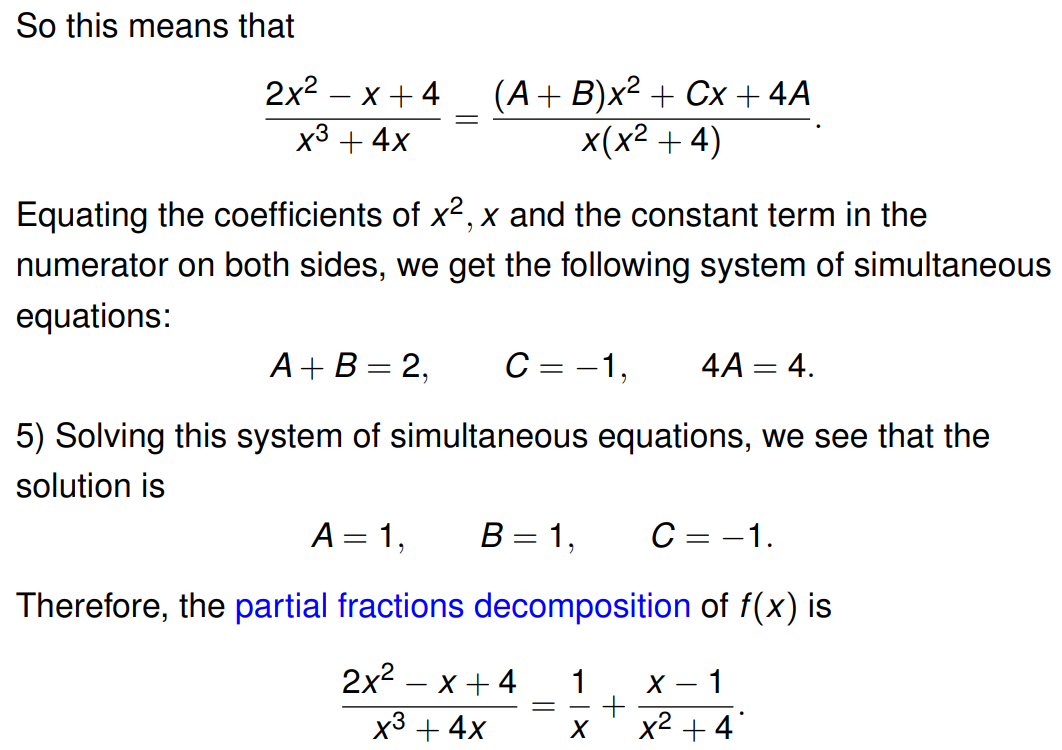
\includegraphics[width=0.59\linewidth]{ex2.png}\\
\textbf{Example: }Find the partial fractions decomposition of $f(x)=\displaystyle\frac{2x+2}{(x^2+1)(x-1)^3}$\\
We can see that $(x^2+1)$ repeats once and $(x-1)$ repeats 3 times.
\begin{flalign*}
  \Rightarrow\ f(x)=&\ \displaystyle\frac{Ax+B}{x^2+1}+\frac{C}{x-1}+\frac{D}{(x-1)^2}+\frac{E}{(x-1)^3}\\
  =&\ \frac{(Ax+B)(x-1)^3+C(x^2+1)(x-1)^2+D(x^2+1)(x-1)+E(x^2+1)}{(x^2+1)(x-1)^3}&&
\end{flalign*}
$=\displaystyle\frac{(A+C)x^4+(-3A+B-2C+D)x^3+(3A-3B+2C-D+E)x^2+(-A+3B-2C+D)x+(-B+C-D+E)}{(x^2+1)(x-1)^3}$\\  
We have these equations:
\begin{align*}
    A+C=0\\
    -3A+B-2C+D=0\\
    3A-3B+2C-D+E=0\\
    -A+3B-2C+D=2\\
    -B+C-D+E=2
\end{align*}
$\Rightarrow\ A=0,B=1,C=0,D=-1,E=2$\\
$\Rightarrow\ f(x)=\displaystyle\frac{1}{x^2+1}-\frac{1}{(x-1)^2}+\frac{2}{(x-1)^3}$ (You can try to determine $I=\int f(x)dx$ to practice)\\
\textbf{Example:} Determine $\displaystyle\int\frac{x^4}{x^2-1}$\\
(This is an improper rational function because the degree of $x^4$ is greater than the degree of $(x^2-1)$)\\
Consider $f(x)=\displaystyle\frac{x^4}{x^2-1}=x^2+1+\frac{1}{x^2-1}$\\
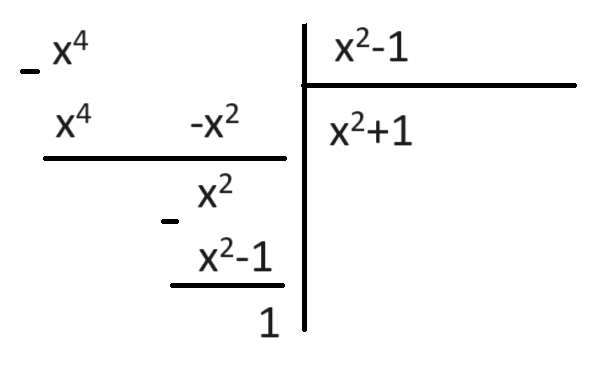
\includegraphics[width=0.5\linewidth]{divi.png}\\
$\Rightarrow\ I=\displaystyle\frac{x^3}{3}+x-ln\left|csc(arcsec\ x)+cot(arcsec\ x)\right|+C$ (hint: substitute x=sec u)\\
\section{Improper Integrals}
\subsection{Type I}
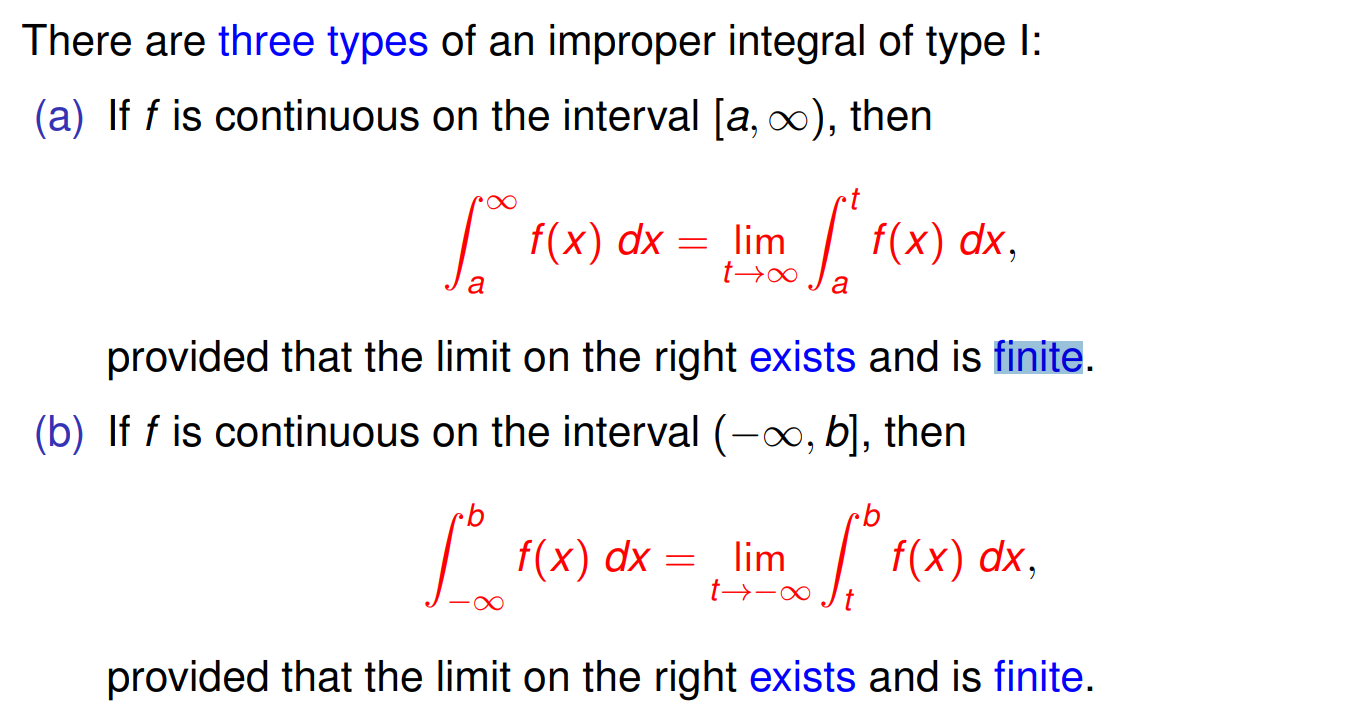
\includegraphics[width=1\linewidth]{tyoe1.png}
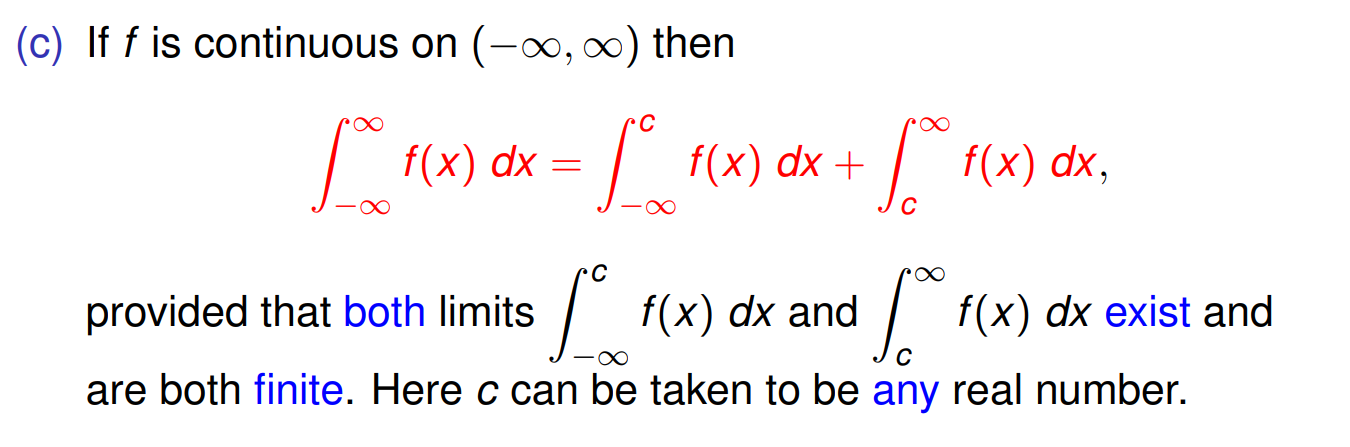
\includegraphics[width=1\linewidth]{type1-2.png}
\textbf{Note: }
\begin{itemize}
    \item $\displaystyle\int\limits_{-\infty}^{\infty}f(x)dx\ne \lim_{x\rightarrow\infty}\int\limits_{-t}^{t}f(x)dx$ 
    \item If the limit is finite and exists, then the corresponding improper integral is convergent (or converges)
    \item If the limit is infinite or does not exist, then the corresponding improper integral is divergent (or diverges)
    \item The improper integral $\displaystyle\int\limits_{1}^{\infty}\frac{1}{x^p}dx$ converges to $\displaystyle\frac{1}{p-1}$ when $p>1$ and diverges when $p\le1$\\
\end{itemize}
\textbf{Example: } Determine whether $I=\displaystyle\int\limits_{0}^{\infty}\frac{dx}{x^2+1}$ converges or diverges\\
$I=\displaystyle\int\limits_{0}^{\infty}\frac{dx}{x^2+1}=\lim_{t\rightarrow \infty}\displaystyle\int\limits_{0}^{t}\frac{dx}{x^2+1}$\\
Let $x=tan\ u\ \left(u\in \left[\displaystyle\frac{-\pi}{2},\frac{\pi}{2}\right]\right)$\\
$\Rightarrow dx=sec^2u\ du$\\
When $x=0\ \Rightarrow\ u=0$\\
.\quad \quad \quad $x=t\ \Rightarrow\ u=arctan\ t$
\begin{flalign*}
I=&\ \displaystyle\lim_{t\rightarrow\infty}\int\limits_{0}^{arctan\ t}\frac{sec^2u\ du}{tan^2u+1}\\
=&\ \lim_{t\rightarrow\infty}\int\limits_{0}^{arctan\ t}\frac{sec^2u\ du}{sec^2u}
=\ \lim_{t\rightarrow\infty}\int\limits_{0}^{arctan\ t}du\\
=&\ \displaystyle\lim_{t\rightarrow\infty}\left[u\right]_{0}^{arctan\ t}=\ \lim_{t\rightarrow\infty}arctan\ t\\
=&\ \frac{\pi}{2}&&
\end{flalign*}
$\Rightarrow$ I converges\\
\textbf{Example: }Determine whether $I=\int\limits_{-\infty}^{0}xe^xdx$ converges or diverges\\
$I=\displaystyle\lim_{t\rightarrow\infty}\int\limits_{-t}^{0}xe^xdx$\\
Applying integration by Parts:\\
Choose $u=x\ \Rightarrow\ du=dx$\\
.\quad\quad\quad  $dv=e^xdx\ \Rightarrow\ v=e^x$
\begin{flalign*}
    \Rightarrow\ I=&\ \displaystyle\lim_{t\rightarrow\infty}\left(\left[xe^x\right]_{-t}^{0}-\int\limits_{-t}^{0} e^xdx\right)\\
    =&\ \displaystyle\lim_{t\rightarrow\infty}(-te^{-t}-\left[e^x\right]_{-t}^{0})\\
    =&\ \displaystyle\lim_{t\rightarrow\infty}\left(\frac{-t}{e^t}-1+\frac{1}{e^t}\right)\\
    =&\ \lim_{t\rightarrow\infty}\frac{-1}{e^t}-1=\ -1&&    
\end{flalign*}
$\Rightarrow$ I converges\\
\newpage
\textbf{Example:} Determine whether $I=\displaystyle\int\limits_{-\infty}^{\infty}\frac{xdx}{(x^2+4)^{3/2}}$ converges or diverges.\\
$I=\displaystyle\lim_{t\rightarrow\infty}\left(\int\limits_{-t}^{0}\frac{xdx}{(x^2+4)^{3/2}}+\int\limits_{0}^{t}\frac{xdx}{(x^2+4)^{3/2}}\right)$\\
Consider $M=\displaystyle\int\frac{xdx}{(x^2+4)^{3/2}}$\\
Let $x=2tan\ u\ \left(u\in \left[\displaystyle\frac{-\pi}{2},\frac{\pi}{2}\right]\right) \\
\Rightarrow\ dx=2sec^2u\ du$
\begin{flalign*}
    \Rightarrow\ M=&\ \displaystyle\int\frac{4tan\ u\ sec^2u\ du}{(4tan^2u+4)^{3/2}}\\
    =&\ \int\frac{4tan\ u\ sec^2u\ du}{4^{3/2}(tan^2u+1)^{3/2}}\\
    =&\ \int\frac{4tan\ u\ sec^2u\ du}{4^{3/2}(sec^2u)^{3/2}}\\
    =&\ \frac{1}{2}\int\frac{tan\ u\ sec^2u\ du}{sec^{3}u}\\
    =&\ \frac{1}{2}\int\frac{tan\ u\ du}{sec\ u}\\
    =&\ \frac{1}{2}\int\frac{\sin\ u\ cos\ u\ du}{cos\ u}\\
    =&\ \frac{1}{2}\int \sin\ u\ du\\
    =&\ -\frac{1}{2}cos\ u+C\\
    =&\ -\frac{1}{2}cos(arctan\frac{x}{2})+C\\
\Rightarrow\ I=&\ \displaystyle\lim_{t\rightarrow\infty}\left(\left[-\frac{1}{2}cos(arctan\frac{x}{2})\right]_{-t}^{0}+\left[-\frac{1}{2}cos(arctan\frac{x}{2})\right]_{0}^{t}\right)\\
=&\ \lim_{t\rightarrow\infty}\left(\frac{-1}{2}+\frac{1}{2}cos(arctan\frac{-t}{2})-\frac{1}{2}cos(arctan\frac{t}{2})+\frac{1}{2}\right)\\
=&\ \frac{1}{2}cos\frac{-\pi}{2}-\frac{1}{2}cos\frac{\pi}{2}=0&&
\end{flalign*}
$\Rightarrow$ I converges\\
\subsection{Type II}
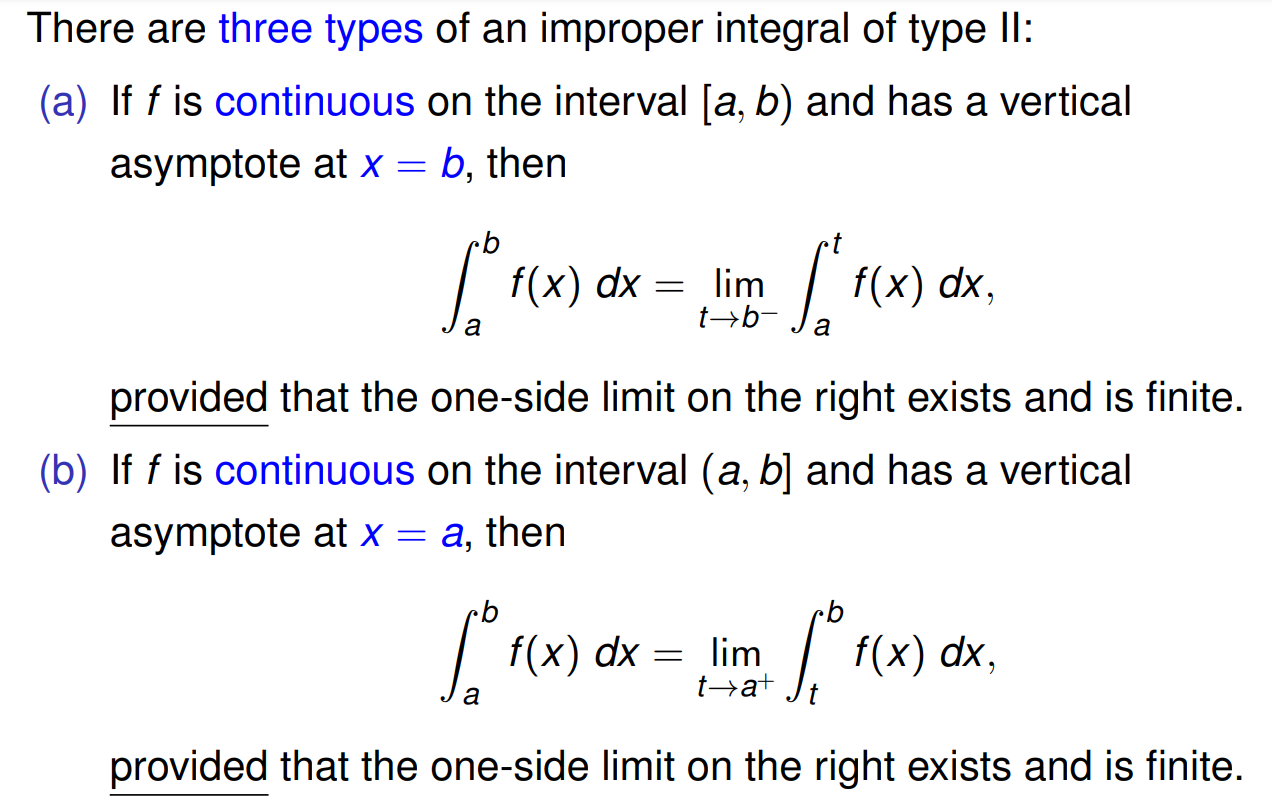
\includegraphics[width=1\linewidth]{type2.png}\\
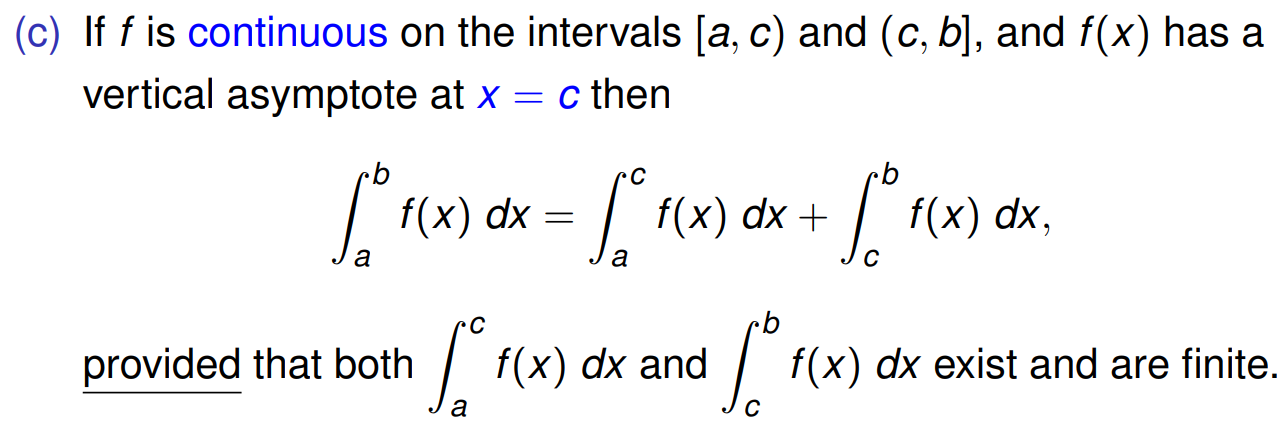
\includegraphics[width=1\linewidth]{type2-2.png}\\
\textbf{Note:}\\
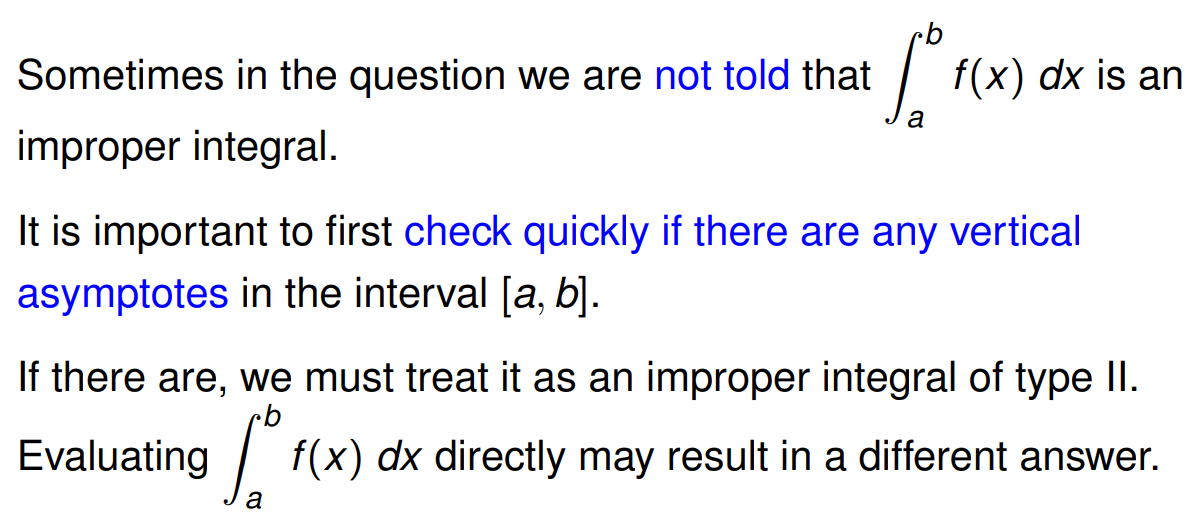
\includegraphics[width=0.7\linewidth]{note.png}\\
\newpage
\textbf{Example: }Determine 
$I=\displaystyle\int\limits_{0}^{\pi/2}cot\ x\ dx$\\
We can see that $f(x)=cot\ x$ is continuous on $\left(0,\displaystyle\frac{\pi}{2}\right]$ and discontinuous at x=0
\begin{flalign*}
    \Rightarrow\ I=&\ \displaystyle\lim_{t\rightarrow 0^+} \int\limits_{t}^{\pi/2}cot\ x\ dx\\
    =&\ \lim_{t\rightarrow 0^+}\left[ln\left|\sin\ x\right|\right]_{t}^{\pi/2}\\
    =&\ \lim_{t\rightarrow 0^+}(-ln\left|\sin\ t\right|)\\
    =&\ -\lim_{t\rightarrow 0^+}ln(\sin\ t)\\
    =&\ -\lim_{t\rightarrow 0^+}ln(t)\\
    =&\ \infty&&
\end{flalign*}
$\Rightarrow$ I diverges\\
\textbf{Example: }Determine $I=\displaystyle\int\limits_{0}^{1}\frac{1}{1-x}dx$\\
We can see that $f(x)=\displaystyle\frac{1}{1-x}$ is continuous on [0,1) and discontinuous at x=1
\begin{flalign*}
    \Rightarrow\ I=&\ \displaystyle\lim_{t\rightarrow 1^-}\int\limits_{0}^{t}\frac{1}{1-x}dx\\
    =&\ \lim_{t\rightarrow 1^-}\left[-ln\left|1-x\right|\right]_{0}
^{t}\\
=&\ -\lim_{t\rightarrow 1^-}ln\left|1-t\right|\\
=&\ -\lim_{t\rightarrow 1^-}ln(1-t)\\
=&\ \infty&&
\end{flalign*}

$\Rightarrow$ I diverges\\
\textbf{Example:} Determine $I=\displaystyle\int\limits_{-1}^{4}\frac{dx}{\sqrt{\left|x\right|}}$\\
We can see that $f(x)=\displaystyle\frac{1}{\sqrt{\left|x\right|}}$ is continuous on $[-1,0)\cup (0,4]$
\begin{flalign*}
    \Rightarrow\ I=&\ \displaystyle\int\limits_{-1}^{0}\frac{dx}{\sqrt{\left|x\right|}}+\displaystyle\int\limits_{0}^{4}\frac{dx}{\sqrt{\left|x\right|}}\\
    =&\ \displaystyle\int\limits_{-1}^{0}\frac{dx}{\sqrt{-x}}+\displaystyle\int\limits_{0}^{4}\frac{dx}{\sqrt{x}}\\
    =&\ \lim_{t\rightarrow 0^-}\int\limits_{-1}^{t}\frac{dx}{\sqrt{-x}}+\lim_{t\rightarrow 0^+}\int\limits_{t}^{4}\frac{dx}{\sqrt{x}}&&
\end{flalign*}
\begin{flalign*}
    =&\ -\lim_{t\rightarrow 0^-}\int\limits_{-1}^{t}(-x)^{-1/2}d(-x)+\lim_{t\rightarrow 0^+}\int\limits_{t}^{4}x^{-1/2}dx\\
    =&\ -\lim_{t\rightarrow 0^-}\left[2(-x)^{1/2}\right]_{-1}^{t}+\lim_{t\rightarrow 0^+}\left[2x^{1/2}\right]_{t}^{4}\\
=&\ -\displaystyle\lim_{t\rightarrow 0^-}\left(2\sqrt{-t}-2\right)+\lim_{t\rightarrow 0^-}\left(4-2\sqrt{t}\right)\\
=&\ 2+4\\
=&\ 6&&
\end{flalign*}
$\Rightarrow$ I converges
\subsection{Comparison Theorem}
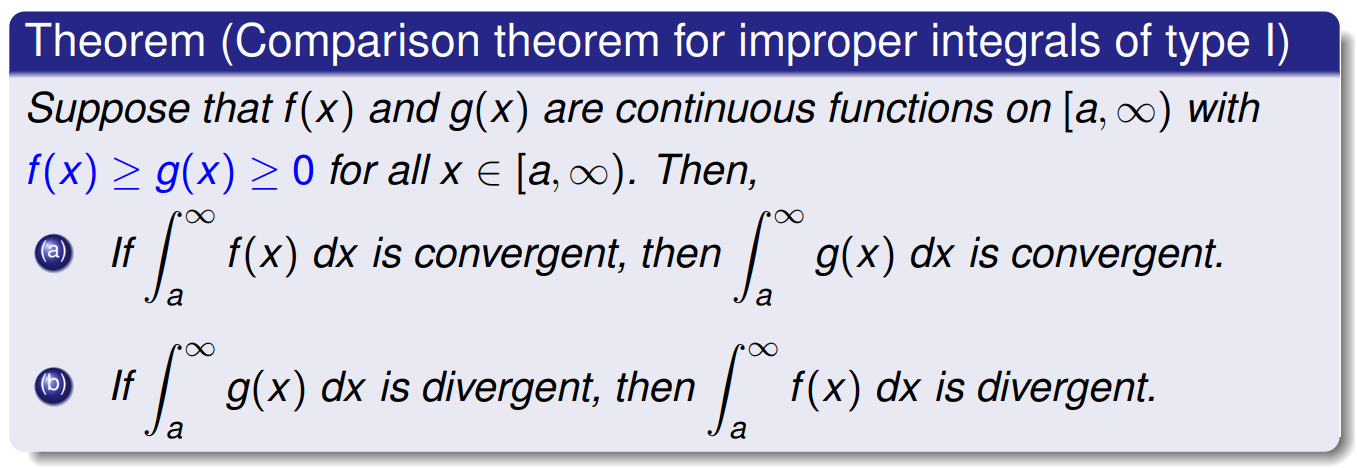
\includegraphics[width=1\linewidth]{compa.png}
\textbf{Example:} Determine whether $\displaystyle\int\limits_{1}^{\infty}\frac{\sin^2x}{x^2}$ converges or diverges\\
We have $0\leq \sin^2x\leq 1$ on $[1,\infty)$\\
$\Rightarrow \displaystyle\frac{0}{x^2}\leq \frac{\sin^2x}{x^2}\leq\frac{1}{x^2}$ on $[1,\infty)$\\
And $\displaystyle\int\limits_{1}^{\infty} \frac{1}{x^2}$ converges\\
$\Rightarrow\ \displaystyle\int\limits_{1}^{\infty}\frac{\sin^2x}{x^2}$ converges\\
$\displaystyle\mathbb{I}$
\end{document}